% プロジェクト学習中間報告書書式テンプレート ver.1.0 (iso-2022-jp)

% 両面印刷する場合は `openany' を削除する
\documentclass[openany,11pt,papersize]{jsbook}

% 報告書提出用スタイルファイル
\usepackage[final]{funpro}%最終報告書
%\usepackage[middle]{funpro}%中間報告書

% 画像ファイル (EPS, EPDF, PNG) を読み込むために
\usepackage[dvipdfmx]{graphicx,color}

% ここから -->
\usepackage{calc,ifthen}
\newcounter{hoge}
\newcommand{\fake}[1]{\whiledo{\thehoge<70}{#1\stepcounter{hoge}}%
  \setcounter{hoge}{0}}
% <-- ここまで 削除してもよい

% 年度の指定
\thisYear{2015}

% プロジェクト名
\jProjectName{フィールドから創る地域・社会のためのスウィフトなアプリ開発}

% [簡易版のプロジェクト名]{正式なプロジェクト名}
% 欧文のプロジェクト名が極端に長い(2行を超える)場合は、短い記述を
% 任意引数として渡す。
%\eProjectName[Making Delicious curry]{How to make delicious curry of Hakodate}
\eProjectName{“Swift” Application Development Based on Field Research}


% <プロジェクト番号>-<グループ名>
\ProjectNumber{3-C}

% グループ名
\jGroupName{教育系グループ}
\eGroupName{Education Group}

% プロジェクトリーダ
\ProjectLeader{1013220}{新保遥平}{Yohei~Shinpo}

% グループリーダ
\GroupLeader  {1013068}{中進吾}{Shingo~Naka}

% メンバー数
\SumOfMembers{5}
% グループメンバ
\GroupMember  {1}{1013130}{熊谷優斗}{Yuto~Kumagai}
\GroupMember  {2}{1013116}{皀勢也}{Seiya~Kurokome}
\GroupMember  {3}{1013220}{新保遥平}{Yohei~Shinpo}
\GroupMember  {4}{1013015}{中進吾}{Shingo~Naka}
\GroupMember  {5}{1013104}{矢吹渓悟}{Keigo~Yabuki}

% 指導教員
\jadvisor{伊藤恵,奥野拓,原田泰,木塚あゆみ,南部美砂子}
% 複数人数いる場合はカンマ(,)で区切る。カンマの前後に空白は入れない。
\eadvisor{Kei~Itou,Taku~Okuno,Yasushi~Harada,Ayumi~Kizuka,Misako~Nanbu}

% 論文提出日
\jdate{2015年7月17日}
\edate{July~17, 2015}

%%%%%%%%%%%%%%%%%%%%%%%%%%%%%%%%%%%%%%%
\usepackage{graphicx}
%%%%%%%%%%%%%%%%%%%%%%%%%%%%%%%%%%%%%%%
\begin{document}
%
% 表紙
\maketitle

%前付け
\frontmatter

% 和文概要
\begin{jabstract} 日本語の概要を書く。
\fake{ここに日本語の概要を書きます。}
% 和文キーワード
\begin{jkeyword}
キーワード1, キーワード2, キーワード3, キーワード4, キーワード5
\end{jkeyword}
\bunseki{未来太郎}
\end{jabstract}

%英語の概要
\begin{eabstract} Abstract in English. 
\fake{you should write your English abstract in one page. }
% 英文キーワード
\begin{ekeyword}
Keyrods1, Keyword2, Keyword3, Keyword4, Keyword5
\end{ekeyword}
\bunseki{函館花子}
\end{eabstract}

\tableofcontents% 目次


\mainmatter% 本文のはじまり

\chapter{背景}
\section{日本のプログラミング教育について}
日本では2012年から中学校の技術家庭科で、プログラミング教育が必修項目となっている。ビジュアルプログラミング言語のScratchやビュートビルダーなどを用いて授業を行っている。また、プログラミングを学ぶのは中学3年生の時だけである。

\bunseki{中進吾}

\section{現状と課題}
中学校ではビジュアル言語を用いた授業を行っており、ソースコードを書く練習はしていない。また、中学校でプログラミングを学べる期間は短い。そのため中学校の授業だけでは、ソースコードを書こうとした時、どのように組んでいいかわからない。
\bunseki{中進吾}

\chapter{本プロジェクトの目標}

\section{目的}\label{sec:mokuteki}
本プロジェクトの目的は、中学校では実際にソースコードを書く練習をしていなく、中学生はソースコードを書こうとした時、どのように組んでいいか分からないため、ソースコードの組み方を学ぶゲームアプリを開発することである。
\bunseki{皀勢也}


\section{目標}
本プロジェクトの目的は、中学校では実際にソースコードを書く練習をしていなく、中学生はソースコードを書こうとした時、どのように組んでいいか分からないため、ソースコードの組み方を学ぶゲームアプリを開発することである。
\bunseki{皀勢也}

%3章
\chapter{プロジェクトの進め方}
\section{イベント}
\subsection{ほげ}
ほげほげ
\bunseki{未来}

\subsection{ほげ}
ほげほげ
\bunseki{未来}

\subsection{ほげ}
ほげほげ
\bunseki{未来}

\subsection{ほげ}
ほげほげ
\bunseki{未来}

\subsection{ほげ}
ほげほげ
\bunseki{未来}

\subsection{ほげ}
ほげほげ
\bunseki{未来}

\section{アプリ案の推移}
ほげほげ
\bunseki{北海}

\chapter{開発アプリについて}
\section{概要}
開発するアプリは中学生を対象としたプログラミングの組み方を学ぶゲームアプリである。
マス目上のステージにある自機をプログラムを組んで動かし、敵機を倒しゴールすることでゲームがクリアとなる。
\bunseki{新保遥平}

\subsection{ゲーム性}
ただプログラミングを学ぶのではなく、ゲームを通してプログラミングを学ぶことでユーザーのモチベーションを保ちつつ、アプリを使ってもらえるのではないかと考えた。また実際に自機をプログラム通りに動かすことが出来たときにプログラミングの学習が深まるのではないかと考えた。
 
\bunseki{新保遥平}

\subsection{教育性}
このアプリではユーザーがソースコードの組み立て方を学ぶことを目的にしている。これを実現するために、このアプリにはコストとランクがある。ソースのボタンそれぞれにコストが設けられており、問題をクリアした際にコストの使用量が少ないほどよいアルゴリズムでソースコードを組み立てることが出来たと判定し、ランクを与える。ランクが低かった場合、より良いランクにつながるヒントを与える。そして高いランクが与えられたときに、ユーザーを褒める言葉を表示する。このサイクルが次の問題への意欲につながる。またより良いアルゴリズムでソースコードを組み立てることが出来るようになる。
\bunseki{新保遥平}

\section{プログラミング画面}

ユーザーは画面左側に配置されたそれぞれのソースボタンをタップして、プログラムを組んでいく。主なソースボタンはattack()、move()、left、right、0〜9などである。タップされたソースボタンは順に、右側のスペースに記述される。例えば下記のようにプログラムを組むことができる。
\par move(left,3);
\par move(up,3);
\begin{flushright}
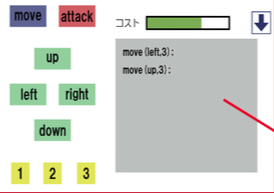
\includegraphics[width=4cm, bb=0 0 274 193]{2015-07-16 22.55.07.jpg}
\end{flushright}


このようなにプログラムをタップで組むことができことが出来る。また、間違ったタイミングでソースボタンを押すと画面上にエラーが出てすぐに確認ができる。

\bunseki{新保遥平}

\section{戦闘画面}
戦闘画面はプログラミング画面で入力したソースコードを実際に動かすための画面である。ソースコードを入力後、戦闘画面にある実行ボタンを押すことで、実機を動かすことが出来る。1回の実行で敵機を倒し、ゴールが出来るようなプログラムを組まなければならない。

\begin{flushright}
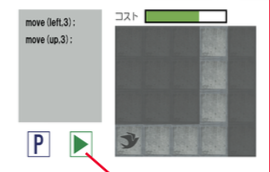
\includegraphics[width=4cm, bb=0 0 274 193]{2015-07-16 23.18.53.jpg}
\end{flushright}




\bunseki{新保遥平}

%5章
\chapter{結果}
\section{プロジェクトの評価}
7月に行われた中間発表会の評価シートの結果から、「声がはっきり聞こえた」、「声は大きく聞きやすかった」などの意見をいただき、発表技術に関しては高い評価を得られた。しかし、発表内容に関しては「最終的なゴールは?」、「まだ内容が決まっていないので評価不能」、「既存のもとの比較がない」などの意見をいただいた。これらの意見をまとめると、私たちのプロジェクトは目標が決まっていなく、内容がわかりづらいという評価であった。
\bunseki{中進吾}

\section{プロジェクトの成果}
小・中学生にプログラミングを教える場合、C言語やJavaから始めるのではなく、Scratchのようなビジュアルプログラミング言語から始めた方が良いということがわかった。また、プログラミングでラジコンやロボットを動かしてもらうことにより、プログラミングに興味を持ってもらうことができるということがわかった。
\bunseki{中進吾}


\chapter{まとめ}
\section{今後の課題と展望}
今後は、現在のアプリ設計案を再考し、より具体的で一貫性がある設計案にしていく必要がある。また、実際にパズルゲームとしての問題を考え、それぞれの答えを用意することや実証実験や評価方法を適切に定める必要がある。
\par
制御文のソースボタンやフィードバック機能を実装し、教育アプリとしての体裁を整え、11月に開催されるアカデミックリンクにてワークショップを開き、そこで得たレビューを活かしてアプリの改善を行うことが今後の展望である。
\bunseki{皀勢也}

\section{学び}
要件定義を固めずに実装を行ったため、プロジェクトの目的を見失い要件定義を一から考え直すことになった。そのため、時間をかけて、要件定義をやり直すことの重要性を学んだ。また、議事録を残していないことがあり、情報共有がうまくできていなかったことからドキュメントを残して、情報共有することの大切さを学んだ。
\bunseki{皀勢也}

% 以降、付録(付属資料)であることを示す
\begin{appendix}

\chapter{新規習得技術}
\begin{hissu}
課題解決過程に習得した技術について解説する。
\end{hissu}

\chapter{活用した講義}
\begin{hissu}
課題解決過程において活用した講義について、講義名・活用内容を記述する。 
\end{hissu}

\chapter{相互評価}
\begin{hissu}
課題解決過程で分担し、連携した作業全般について、互いに客観的に評価する。 
\end{hissu}

\chapter{その他製作物}
\begin{hissu}
その他成果物をプロジェクトの担当教員の指示に従って添付する。
\end{hissu}

%付録の終わり
\end{appendix}


%\backmatter

% 参考文献
\begin{thebibliography}{9}
 \bibitem {ラベル} 著者名. 書籍名. 出版社,  年号.
 \bibitem {A2} ほげほげお. うんたらかんたら,  2003.
\end{thebibliography}

\end{document}